\section{Homogeneous Transformations}
\subsection*{Dilatation}
\smallskip

\textbf{Homogeneous Dilatation:} {$\tensor[^i]{\underline{\mathbf{y}}}{} = \lambda (t/t_{max}) {\underline{\underline{\mathbf{I}}}} \tensor[^i]{\underline{\mathbf{x}}}{} \qquad i = 1,4 $} \\
with $ {\underline{\underline{\mathbf{I}}}} = \left[\begin{array}{ccc}1 & 0 & 0 \\0 & 1 & 0 \\0 & 0 & 1\end{array}\right]$
\lstinputlisting[style=Matlab-editor,basicstyle=\color{black}\ttfamily\normalsize, firstline=7, lastline=11]{CheatSheet.m}

\subsection*{Deformations}
\smallskip

\textbf{Uniaxial Deformation:}  {$\tensor[^i]{\underline{\mathbf{y}}}{}(t) = \underline{\underline{\mathbf{U}}} (t/t_{max})\tensor[^i]{\underline{\mathbf{x}}}{} \qquad i = 1,4 $} \\
$ \underline{\underline{U}}(t) = \underline{\underline{I}} + (\upsilon_a(t) -1) \underline{e}_1 \otimes \underline{e}_1 $ \\
with $ \underline{\underline{\mathbf{U}}} = \left[\begin{array}{ccc}1 & 0 & 0 \\0 & 1 & 0 \\0 & 0 & 2+t\end{array}\right]$ in case of a $300 \%$ deformation along $\tensor[^3]{e}{}$.
\smallskip

\textbf{Shear Deformation:}  {$\tensor[^i]{\underline{\mathbf{y}}}{}(t) = \underline{\underline{\mathbf{G}}} (t/t_{max})\tensor[^i]{\underline{\mathbf{x}}}{} \qquad i = 1,4 $} \\
Apply shear deformation ${\underline{\underline{\mathbf{G}}}}$ of ${\frac{\pi}{3}}$ along the vectors  $\tensor[^1]{e}{} - \tensor[^2]{e}{}$ linearly in time.
With det$\underline{\underline{\mathbf{G}}} = 1$ and $\underline{\underline{\mathbf{G}}} \neq \tensor[]{\underline{\underline{\mathbf{G}}}}{^T}$, which means that $\underline{\underline{\mathbf{G}}}$ contains a rotation.
\smallskip

\textbf{Simple shear:} $\underline{\underline{\mathbf{G}}}(t) = \underline{\underline{I}} + \tan{(\gamma (t))} (\underline{p} \otimes \underline{q})$ \\
$ \underline{\underline{\mathbf{G}}}(t) = \left[\begin{array}{ccc}1 & \tan (\gamma) & 0 \\0 & 1 & 0 \\0 & 0 & 1\end{array}\right]$ \\
$ \det{\underline{\underline{\mathbf{G}}}} = 1 \rightarrow $ no change of volume, rotation!

\textbf{Pure shear:} $\underline{\underline{U}} = \underline{\underline{U}}^T \rightarrow $ no rotation! \\
$ \underline{\underline{\mathbf{G}}}(t) = \left[\begin{array}{ccc}1 & \frac{1}{2} \tan (\gamma) & 0 \\ \frac{1}{2} \tan (\gamma) & 1 & 0 \\0 & 0 & 1\end{array}\right]$ \\

\textbf{General Deformation:} \\
Volume change: $V_t = \operatorname{det}(\underline{\underline{\mathbf{F}}}) V $ \\
Area-weighted normals of the tetrahedron: 
$\tensor[^i]{A}{_t} \tensor[^i]{\underline{\mathbf{n}}}{_t} = \operatorname{det}(\underline{\underline{\mathbf{F}}}) \tensor[]{\underline{\underline{\mathbf{F}}}}{^{-T}} \tensor[^i]{A}{} \tensor[^i]{\underline{\mathbf{n}}}{}$
\smallskip
Apply general deformation: {$\tensor[^i]{\underline{\mathbf{y}}}{}(t) = \underline{\underline{\mathbf{F}}} (t/t_{max})\tensor[^i]{\underline{\mathbf{x}}}{} \qquad i = 1,4 $}\\
Where $\underline{F}$ is the Fréchet derivative of a motion (represents rotation, deformation, translation). \\

\textbf{Gradient of transformation:} The infinitesimal transformations of a fiber $da$, surface $ds$ and volume $dV$ are given by: \\

$ d \underline{a}_t = \underline{\underline{F}} d \underline{a} $ \\
$ d \underline{s}_t = J \underline{\underline{F}} ^{-T} d \underline{s} = \underline{\underline{F}}^* d \underline{s}$ \\
$ d V_t = \det{\underline{\underline{F}}} dV = JdV $ \\
With $F^* = j \cdot \underline{\underline{F}} ^{-T} =  \det({\underline{\underline{F}}}) \cdot \underline{\underline{F}} ^{-T}$ \\

$\underline{\underline{\mathbf{F}}}(\underline{\mathbf{x}},t) = \underline{\underline{\mathbf{H}}}(\underline{\mathbf{x}},t) + \underline{\underline{\mathbf{I}}} = \left[\begin{smallmatrix} \frac{\delta y_1}{\delta x_1} & \frac{\delta y_1}{\delta x_2} & \frac{\delta y_1}{\delta x_3} \\ \frac{\delta y_2}{\delta x_1} & \frac{\delta y_2}{\delta x_2} & \frac{\delta y_2}{\delta x_3} \\ \frac{\delta y_3}{\delta x_1} & \frac{\delta y_3}{\delta x_2} & \frac{\delta y_3}{\delta x_3} \end{smallmatrix}\right]$ \\

\medskip
Properties of $ \mathbf{\underline{\underline{F}}}: $
\begin{enumerate}
\item $ \underline{\underline{F}} \neq \underline{\underline{F}}^T $: usually \underline{\underline{F}} is not symmetric.
\item $0 < \det{\underline{\underline{F}}} < \infty $
\item $\underline{\underline{F}}^{-1} \underline{\underline{F}} = \underline{\underline{I}}$
\item if $J(\underline{\mathbf{x}},t) = 1$, $\rightarrow$ \textbf{incompressible} (isochoric)
\end{enumerate}
The Jacobian $J(x,t)$ of the transformation is the change of volume of an infinitesimal element at point \underline{x}. \\

\textbf{Cayley-Hamilton} claims that each tensor of Order 2 satisfies: \\
$\underline{\underline{\mathbf{F}}}^3 - \Tr({\underline{\underline{\mathbf{F}}}}) \underline{\underline{\mathbf{F}}}^2 + \Sec({\underline{\underline{\mathbf{F}}}}) \underline{\underline{\mathbf{F}}} - \det({\underline{\underline{\mathbf{F}}}}) \underline{\underline{\mathbf{I}}} = \underline{\underline{\mathbf{0}}}$ \\
The 3 consecutive powers of $\underline{\underline{\mathbf{F}}}$ having the same eigenvectors are related by their singular values. \\

\textbf{Polar Decomposition:} $ \underline{\underline{F}} = \underline{\underline{R}} \underline{\underline{U}} = \underline{\underline{V}} \underline{\underline{R}} $, where: \\
$\underline{\underline{U}}$ : \textbf{right} stretch tensor (pos, def, symm.) $ \hspace{8mm} \sqrt{\underline{\underline{F}}^T \underline{\underline{F}}} $ \\ 
$\underline{\underline{V}}$ : \textbf{left} stretch tensor (pos, def, symm.) $ \hspace{10mm} \sqrt{\underline{\underline{F}} \underline{\underline{F}}^T} $ \\

\begin{center}
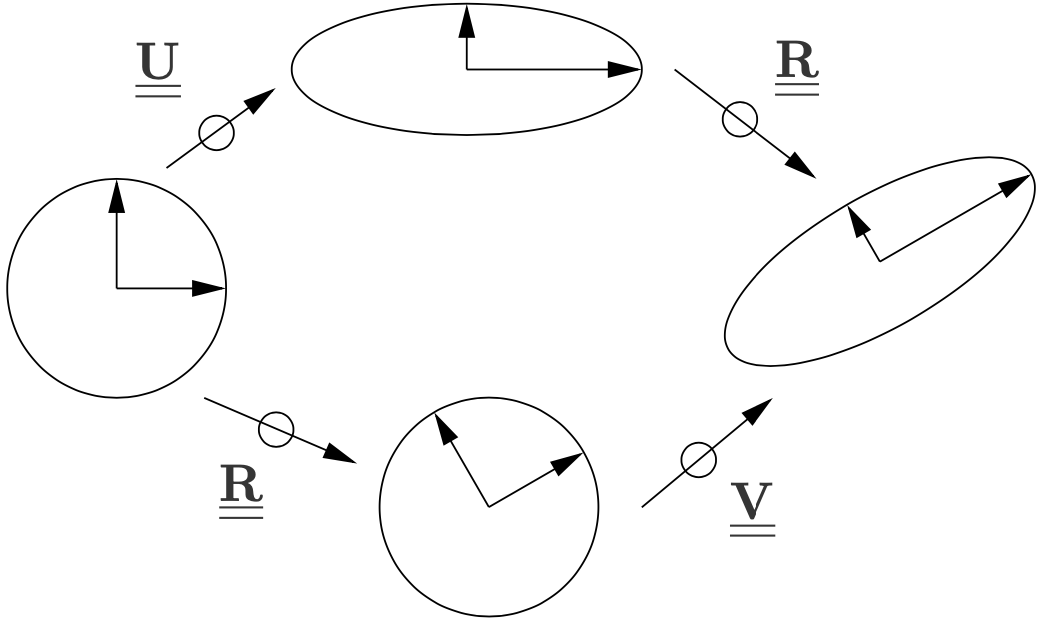
\includegraphics[width=0.6\linewidth]{img/PolarDecomp} \\
\end{center}

\textbf{Singular decomposition:} $ \underline{\underline{F}} =  \sum_{a=1}^{3} \upsilon_a (\underline{b}_a \otimes \underline{c}_a) $, with: \\
$\upsilon_a$: singular values of $\underline{\underline{F}}$ \quad $ 0 < \upsilon_a < \infty$ \quad $\underline{b}_a = \underline{\underline{R}} \underline{c}_a $ \quad $ \underline{c}_a \cdot \underline{c}_b = \delta_{ab} $ \\

The \textbf{invariants} of the gradient of the transformation can be expressed in terms of the singular values: \\
$\Tr{\underline{\underline{F}}(\underline{x},t)} = \sum_{a=1}^{3} \upsilon_a$ \\
$\Sec{\underline{\underline{F}}(\underline{x},t)} = \sum_{a=1}^{3} \upsilon_a \upsilon_b $ \\
$\det{\underline{\underline{F}}(\underline{x},t)} = \prod_{a=1}^{3} \upsilon_a $ \\


\textbf{Spectral decomposition:} states that a symmetric, strictly positive definite tensor ${\underline{\underline{\mathbf{U}}}}$ can be expressed as:

${\underline{\underline{\mathbf{U}}}} = \sum \limits_{a=1}^{3} v_a (\mathbf{\underline{c}}_{a} \otimes \mathbf{\underline{c}}_{a})$ \\

\textbf{Unimodular decomposition:} states that ${\underline{\underline{\mathbf{F}}}}$ can be decomposed in a spherical compression or dilatation ${\underline{\underline{\mathbf{J}}}}$ and an isovolumic deformation ${\underline{\underline{\mathbf{\hat{F}}}}}$ \\

${\underline{\underline{\mathbf{F}}}} = {\underline{\underline{\mathbf{J}}}} {\underline{\underline{\mathbf{\hat{F}}}}} = {\underline{\underline{\mathbf{\hat{F}}}}} {\underline{\underline{\mathbf{J}}}}$ \\
${\underline{\underline{\mathbf{J}}}} = J^{\frac{1}{3}}  {\underline{\underline{\mathbf{I}}}}$ \\


\textbf{Infinitesimal Strain tensor:} \\
${\underline{\underline{\mathbf{\epsilon}}}} = \frac{1}{2}({\underline{\underline{\mathbf{H}}}}+{\underline{\underline{\mathbf{H}}}}^T)$ \\
Relative volume change is approximated by: \\
$\frac{\Delta V}{V} \cong \Tr({{\underline{\underline{\mathbf{\epsilon}}}}})$
